%%%%%%%%%%%%%%%%%%%%%%%%%%%%%%%%%%%%%%%%%
% Ay 190 - WS2
% Written by Chatarin Wong-u-railertkun
%%%%%%%%%%%%%%%%%%%%%%%%%%%%%%%%%%%%%%%%%

%----------------------------------------------------------------------------------------
%	PACKAGES AND OTHER DOCUMENT CONFIGURATIONS
%----------------------------------------------------------------------------------------

\documentclass[11pt,letterpaper]{article}

% Load some basic packages that are useful to have
% and that should be part of any LaTeX installation.
%

\usepackage{graphicx}     % be able to include figures

\usepackage{xcolor}         % get nice colors

% change default font to Palatino (looks nicer!)
\usepackage[latin1]{inputenc}
\usepackage{mathpazo}
\usepackage[T1]{fontenc}

% load some useful math symbols/fonts
\usepackage{latexsym,amsfonts,amsmath,amssymb}
\usepackage{subcaption}

% comfort package to easily set margins
\usepackage[top=1in, bottom=1in, left=1in, right=1in]{geometry}

% control some spacings
%
% spacing after a paragraph
\setlength{\parskip}{.15cm}
% indentation at the top of a new paragraph
\setlength{\parindent}{0.0cm}

\usepackage{courier}


%----------------------------------------------------------------------------------------
%	TITLE
%----------------------------------------------------------------------------------------

\begin{document}

\begin{center}
\Large
Ay190 -- Worksheet 09 - LSE \\    %%%%%% DON'T FORGET TO CHANGE THE WORK SHEET NUMBER
Chatarin (Mee) Wong-u-railertkun\\
Date: \today
\end{center}

\section{Is the system solvable?}
We read the data of A matrix and $\mathbf{b}$ vector. In order of the system to be solvable, $det(A) \neq 0$, $\mathbf{b} \neq \mathbf{0}$, and, the size of A and b must be compatible. First, after importing data into \texttt{Numpy} array, I make sure that b is not equal to zero vector. In table \ref{tab:solvable}, we can see that all the linear equation systems are solvable. (Even though python spits out Overflow while it tries to calculate some determinant, it's not a problem, yet, since Overflow means that the determinant is not zero.)

\begin{table}[h!]
	\centering
	\begin{tabular}{r || r | r | r}
		% Table Header
		i & size(A) & size (b) & det(A) \\
		\hline
		\hline
		1 & (10, 10) & (10,) & 0.0107420716256 \\
		2 & (100, 100) & (100,) & -3.083846412324e+33 \\
		3 & (200, 200) & (200,) & -1.51714199214e+98 \\
		4 & (1000, 1000) & (1000,) & Overflow (-inf) \\
		5 & (2000, 2000) & (2000,) & Overflow (+inf) \\
		\hline
	\end{tabular}
	\caption{The table shows size of A matrix and b vector, and det(A). Since, for all the systems, the size of A and b are compatible, and det(A) are not equal to zero, they are all solvable.}
	\label{tab:solvable}
\end{table}

\section{Gaussian Elimination}
I use \texttt{scipy.linalg.lu} to perform the Gaussian elimination. Then, I wrote a function to solve the linear system. In order to test the function, I randomly generated 3x3 A matrix and vector x of length 3. Multiply both of them to find b, and input A and b into the linear equations solver function. Then, by comparing the error between the generated x and the result from the solver function, we can see how good the Gaussian Elimination method is. Table \ref{tab:GaussError} shows absolute error being very close to zero.

\begin{table}[h!]
	\centering
	\begin{tabular}{| r | r |}
		% Table Header
		Index & Absolute error \\
		\hline
		\hline
		1 & 1.11022302e-16 \\
		2 & 3.33066907e-16 \\
		3 & 3.33066907e-16 \\
		\hline
	\end{tabular}
	\caption{The table shows absolute error between the analytical answer of x and the x from linear equation solver using Gaussian Elimination.}
	\label{tab:GaussError}
\end{table}

\section{Computing Time}
Comparing time taken to solve linear equations of different size, with the Gaussian Elimination method and \texttt{Numpy.linalg.solve}, which uses LAPACK routine \_gesv

\begin{figure}[h!]
	\centering
	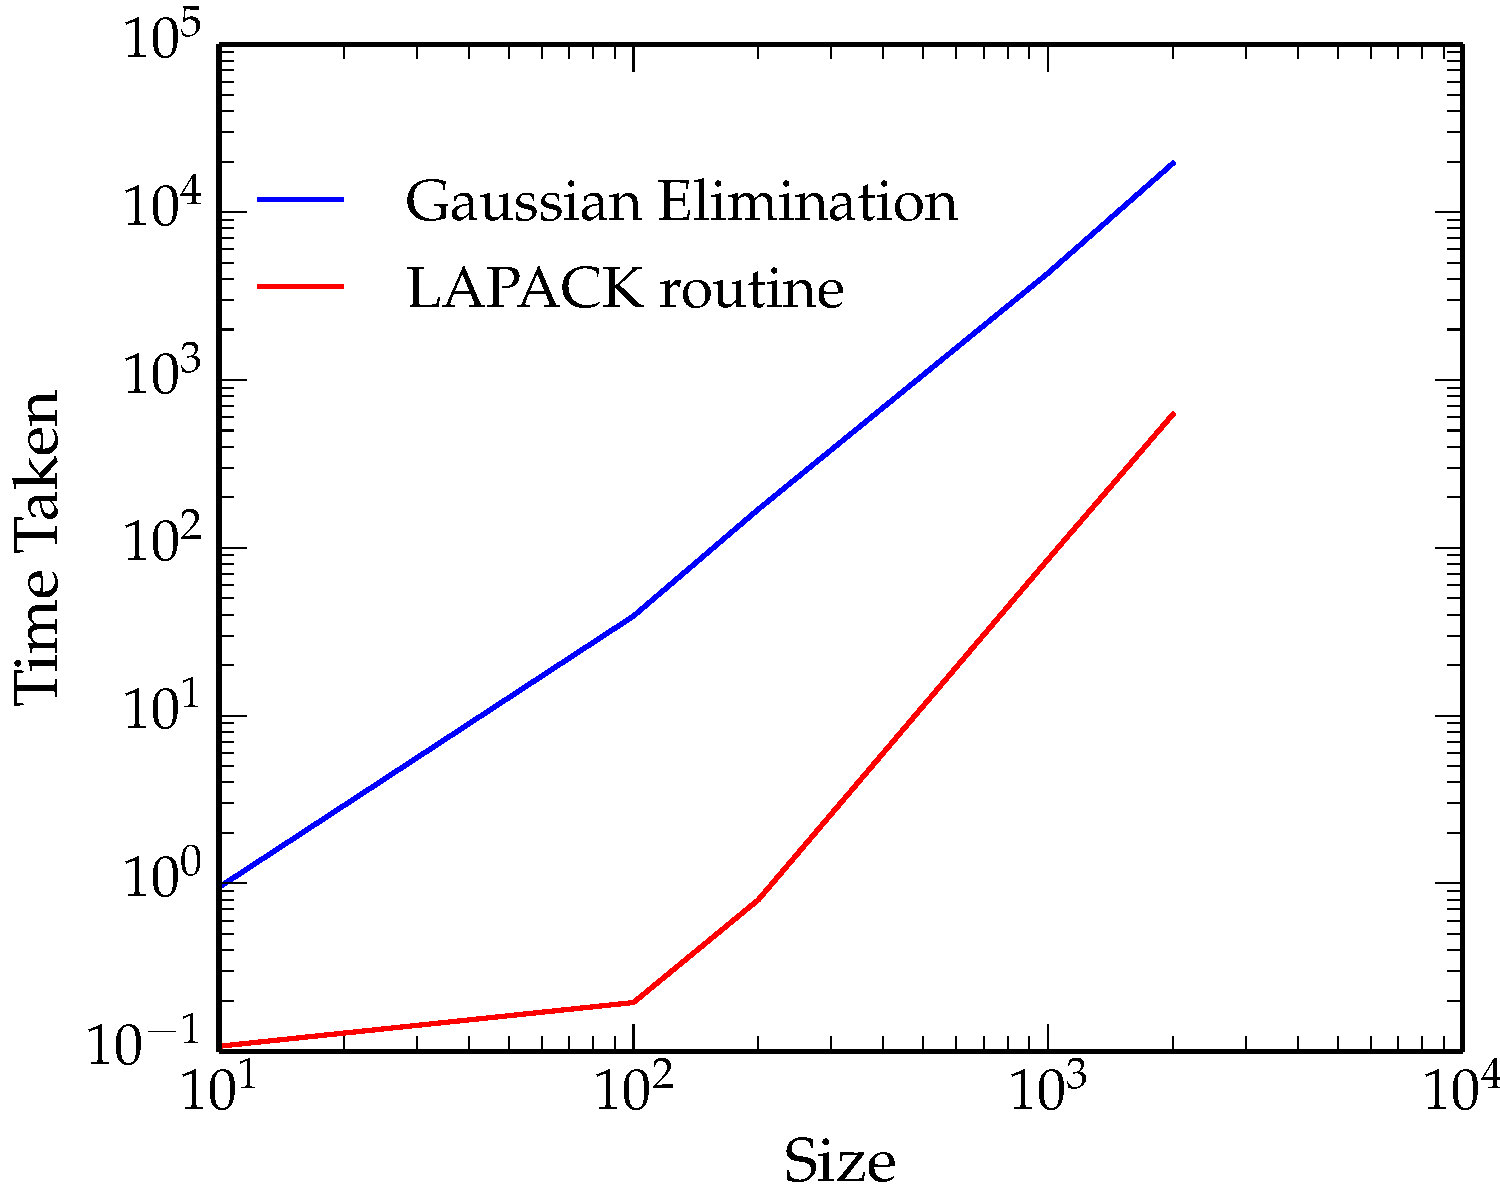
\includegraphics[width=0.5\textwidth]{TimeTaken}
	\caption{Time used to solve linear equations of different sizes with two methods.}
	\label{fig:TimeTaken}
\end{figure}

\end{document}

